\documentclass[compress]{beamer}
\setbeamertemplate{section in toc}[sections numbered]
\usepackage{verbatim}
\usepackage{algorithmic}
\usepackage{mathtools}
\usepackage{xcolor, graphicx}
\newcommand{\x}{{\mathbf x}}
\newcommand{\z}{{\mathbf z}}
\newcommand{\y}{{\mathbf y}}
\newcommand{\w}{{\mathbf w}}
\newcommand{\W}{{W}}
\newcommand{\E}{{E}}
\renewcommand{\l}{{^l}}
\newcommand{\lplus}{{^{l+1}}}
\newcommand{\lminus}{{^{l-1}}}
\definecolor{Blue}{rgb}{0.3,0.3,0.9}
\definecolor{Red}{rgb}{0.9,0.3,0.3}
\newcommand{\textbblue}[1]{{\bf\color{Blue} #1}}
\newcommand{\textbred}[1]{{\bf\color{Red} #1}}
\newcommand{\is}[1]{\setlength{\itemsep}{#1}}
\renewcommand{\Re}{{\mathbb R}}
\DeclareMathOperator*{\argmin}{arg\,min}
\DeclareMathOperator*{\argmax}{arg\,max}


\author{
   		Thomas Hofmann \\[5mm] 
		Institute for Machine Learning \\ ETH Zurich
	} 

\title{
		Advances in Deep Learning Models \\ for Cosmology
	}

\date{
		June 10, 2019
	}

\begin{document}

\frame[plain]{\titlepage}

%%%%%%%%%%%%%%%%%%%%%%%%%%%%%%%%%%%%%%%%
%%%%%%%%%%%%%%%%%%%%%%%%%%%%%%%%%%%%%%%%
\section{Deep Convolutional Networks}
\frame{\sectionpage}
%%%%%%%%%%%%%%%%%%%%%%%%%%%%%%%%%%%%%%%%
%%%%%%%%%%%%%%%%%%%%%%%%%%%%%%%%%%%%%%%%


%%%%%%%%%%%%%%%%%%%%%%%%%%%%%%%%%%%%%%%%
\begin{frame} \frametitle{Deep Neural Networks}
%%%%%%%%%%%%%%%%%%%%%%%%%%%%%%%%%%%%%%%%
\begin{center}
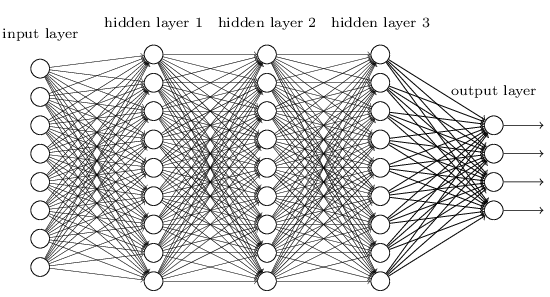
\includegraphics[width=0.52\textwidth]{./figures/OH3gI.png}
\end{center}

Layer-to-layer maps: \textbblue{generalized linear} % (= lin.~+ pointw.~non-lin.)
\begin{align*}
\x^+ = \sigma \left( \W \, \x \right), \quad x^+[i] = \sigma\left(\sum_{j} \W[i,j]\, \, x[j]\right)\in\Re
\end{align*}
\vspace*{-5mm}
\begin{itemize}
\item $\sigma$: fixed activation function(s) (e.g.~ReLU, sigmoid)
\item $\W$: adaptable weight matrix(-ices)
\item layers $l=1\dots L$ (\textbred{depth}), $i=1\dots n[l]$ (\textbred{width}).\\[2mm]
\end{itemize}
\end{frame}

%%%%%%%%%%%%%%%%%%%%%%%%%%%%%%%%%%%%%%%%
\begin{frame} \frametitle{Convolutional Layers: 1D, 2D}
%%%%%%%%%%%%%%%%%%%%%%%%%%%%%%%%%%%%%%%%

Convolutional layer = (discrete) \textbblue{cross-correlation} of signals 
\begin{align*}
\y= \w \star \x, \quad   y[t] \; = \sum_{\Delta t=-m}^m w[\Delta t] \,\, x[t+\Delta t]
\end{align*}
\vspace*{-2mm}
\begin{itemize} \is{2mm}
\item $w[-m\!:\!m]$: filter mask or kernel of width $2m+1$
\item $\y = \W \,\x$, where $\W$ is a bandwidth-limited Toeplitz matrix
\item parameter sharing ($\equiv$ \textbblue{shift invariance})
\end{itemize}
\vspace*{3mm}
Generalize to 2D (or 3D, or any dimensionality)
\begin{align*}
\y & = \w \star \x, \quad y[s,t]  = \sum_{\Delta s} \sum_{\Delta t} w[\Delta s,\Delta t] \; x[s+\Delta s, t+\Delta t ] 
\end{align*}
\end{frame}


%%%%%%%%%%%%%%%%%%%%%%%%%%%%%%%%%%%%%%%%
\begin{frame} \frametitle{Convolutional Networks: ConvNets}
%%%%%%%%%%%%%%%%%%%%%%%%%%%%%%%%%%%%%%%%
Convolutional networks: \textbred{multiple, stacked feature maps}
\begin{align*}
\underbrace{y[r]}_{\substack{\text{$r$-th} \\ \text{channel}}}[s,t] = \sum_{u} \sum_{\triangle s, \triangle t}  \underbrace{w[r,u][\triangle s, \triangle t]}_{\text{parameters}} \underbrace{x[u]}_{\substack{\text{$u$-th}\\\text{channel}}}[s+\triangle s,t + \triangle t]
% y & = \w \star \x, \quad y[s,t]  = \sum_{\Delta s} \sum_{\Delta t} w[\Delta s,\Delta t] \; x[s+\Delta s, t+\Delta t ] 
\end{align*}

\begin{itemize} \is{2mm}
\item $\x, \y$ tensor, $3$-rd order
\item number of parameters $\underbrace{\#r \cdot \#u}_{\text{fully connected}} \cdot \;\underbrace{\#\triangle s \cdot \# \triangle t}_{\text{window size}}$
\item pointwise non-linearities (e.g.~ReLU) 
\item interleaved with: pooling (e.g~max, average)
\item optionally: downsampling (use of strides)
\end{itemize}
\end{frame}

%%%%%%%%%%%%%%%%%%%%%%%%%%%%%%%%%%%%%%%%
\begin{frame} \frametitle{AlexNet}
%%%%%%%%%%%%%%%%%%%%%%%%%%%%%%%%%%%%%%%%
{\small \textit{Krizhevsky, Sutskever, Hinton: Imagenet classification with deep convolutional neural networks. NIPS 2012. [40k+cit]}}
\begin{center}
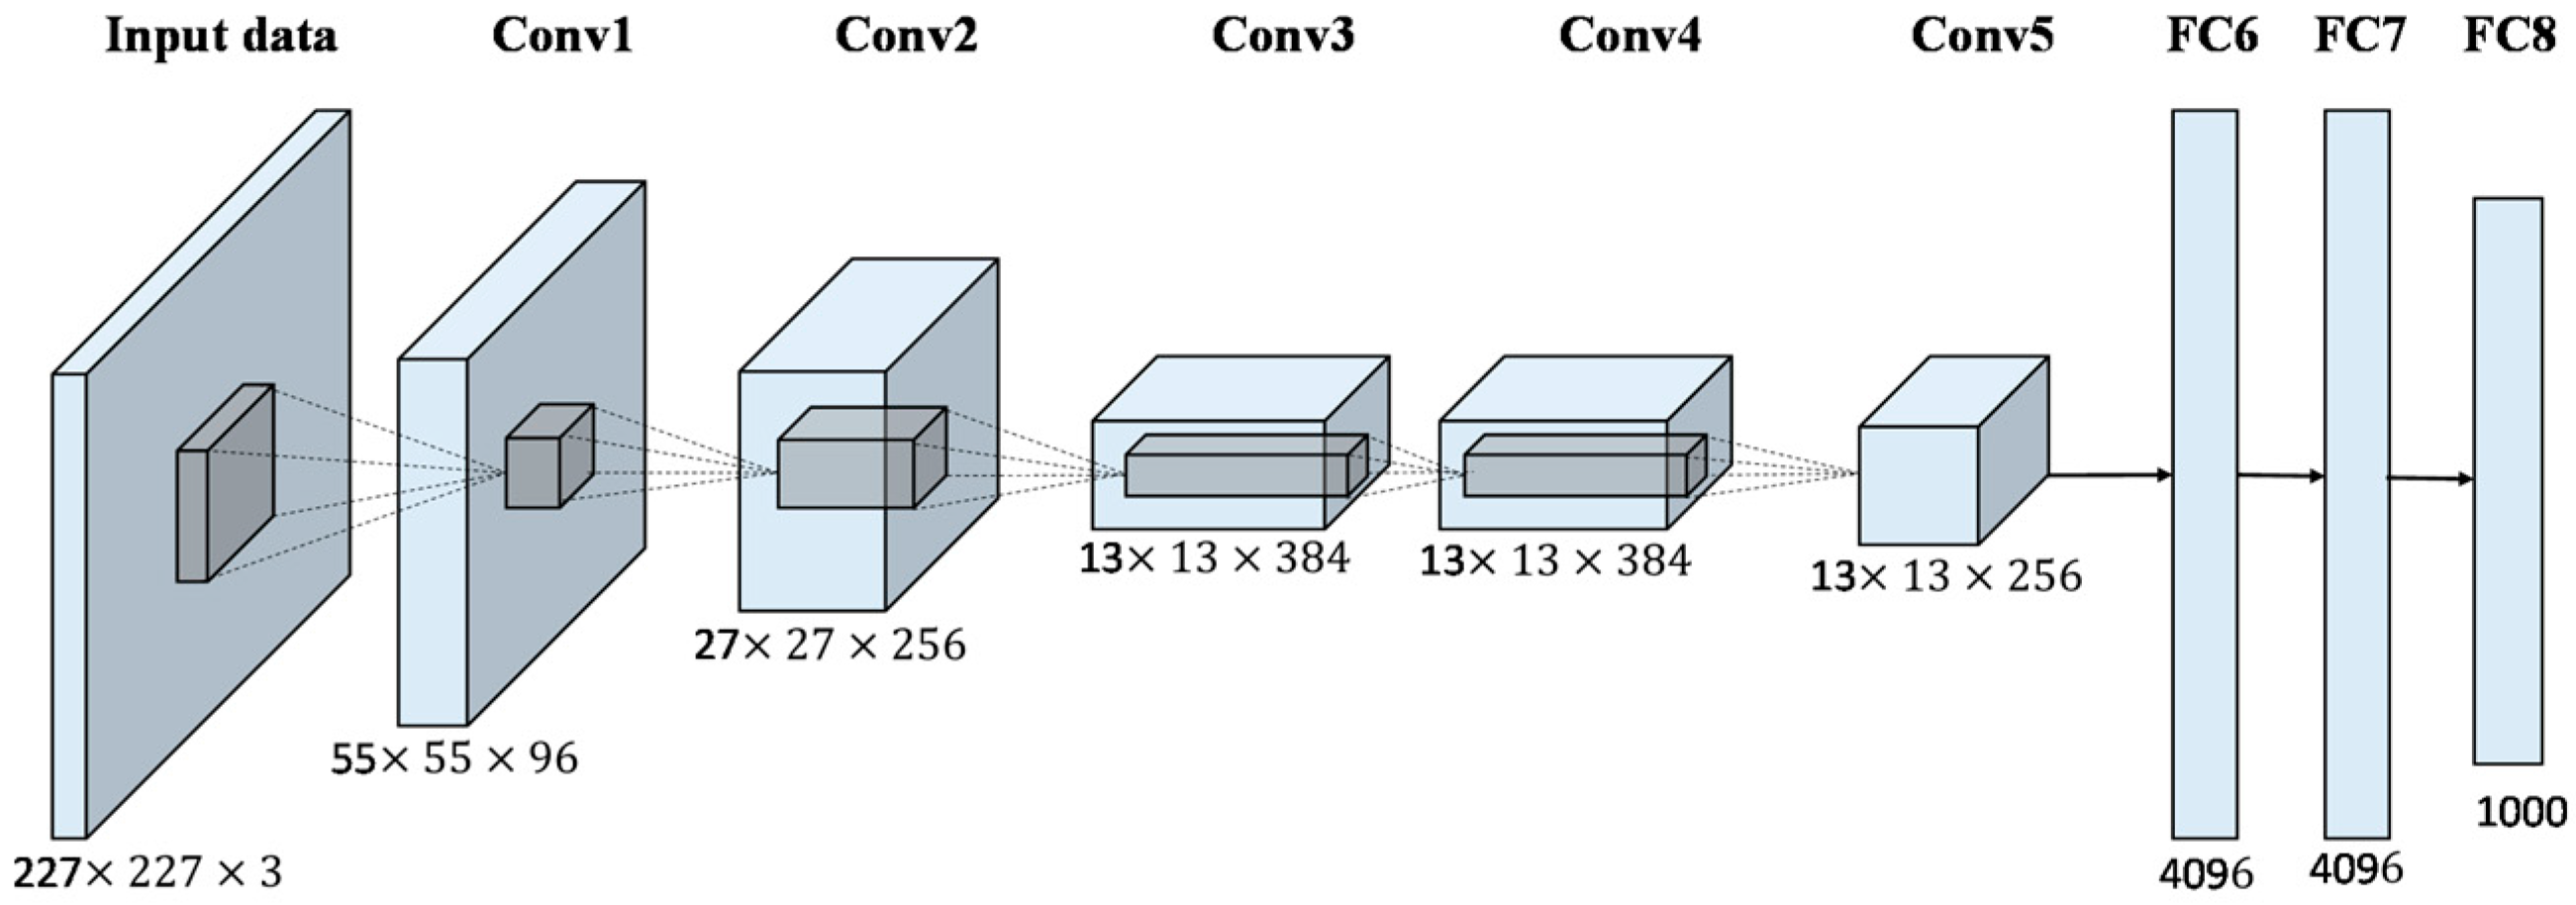
\includegraphics[width=0.66\textwidth]{./figures/alexnet.png}
\end{center}
\begin{itemize} \is{2mm}
\item \textbblue{Pyramidal architecture}: reduce spatial resolution, increase channels with depth
\item Challenge: many channels (width) +large windows +depth
\item Number of parameters\\[1mm]
\begin{itemize}\is{1mm}
\item $384$ to $384$ channels with  $3 \times 3$ window: $>1.3$ M
\item $13 \times 13 \times 384$ tensor to $4096$, fully connected: $>265$ M
\end{itemize}
\end{itemize}
\end{frame}

%%%%%%%%%%%%%%%%%%%%%%%%%%%%%%%%%%%%%%%%
\begin{frame} \frametitle{Deep ConvNets: Key Challenges}
%%%%%%%%%%%%%%%%%%%%%%%%%%%%%%%%%%%%%%%%
\begin{itemize} \is{3mm}
\item Avoid blow-up of model size (e.g.~\# parameters)
\item Preserve computational efficiency of learning (e.g.~gradients)
\item Allow for large depth (\textit{as it is known to be a plus})
\item Allow for sufficient width (\textit{as it is known to be a plus, too})
\end{itemize}
\end{frame}

%%%%%%%%%%%%%%%%%%%%%%%%%%%%%%%%%%%%%%%%
\begin{frame} \frametitle{Very Deep Convolutional Networks: VGG}
%%%%%%%%%%%%%%%%%%%%%%%%%%%%%%%%%%%%%%%%
\begin{columns}
\begin{column}{0.48\textwidth}
{\small \textit{Simonyan, Zisserman: Very deep convolutional networks for large-scale image recognition. ICLR 2015 [23k+cit]}}
\end{column}
\begin{column}{0.50\textwidth}
\begin{center}
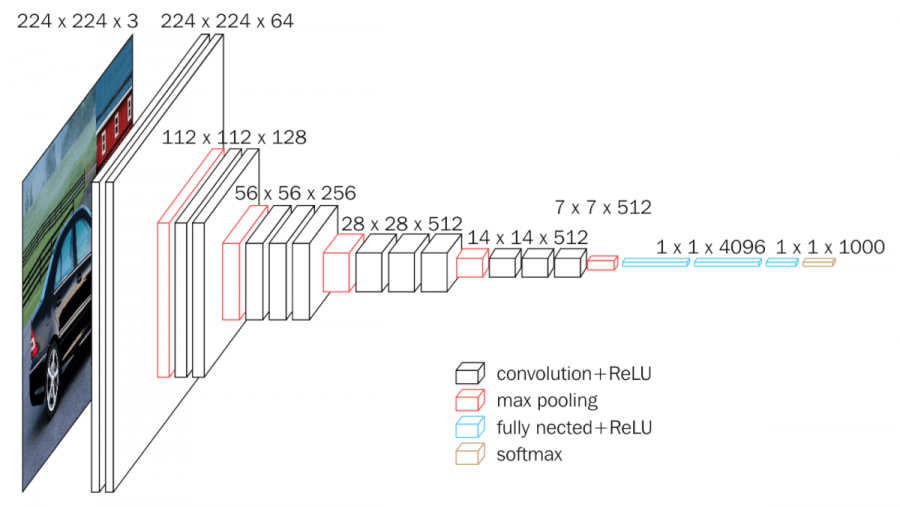
\includegraphics[width=0.99\textwidth]{./figures/vgg.png}
\end{center}
\end{column}
\end{columns}
\begin{itemize} \is{2mm}
\item use very small receptive fields (maximally $3 \times 3$)
\item avoid downsampling/pooling
\item stacking small receptive fields: more depth, fewer parameters
\item example: $3 \cdot (3 \times 3) = 27 < 49= (7 \times 7)$
\end{itemize}
\end{frame}

%%%%%%%%%%%%%%%%%%%%%%%%%%%%%%%%%%%%%%%%
\begin{frame} \frametitle{Network within Network}
%%%%%%%%%%%%%%%%%%%%%%%%%%%%%%%%%%%%%%%%
{\small \textit{Lin, Chen, Yan: Network in network. arXiv:1312.4400, 2013 [2.5k+cit]}}
\begin{center}
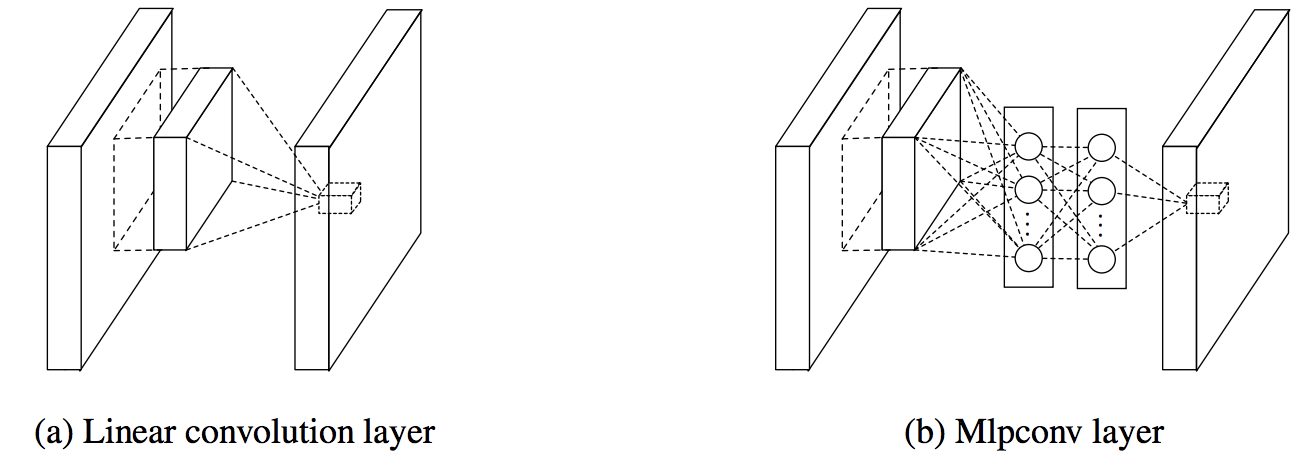
\includegraphics[width=0.8\textwidth]{./figures/netinnet.png}
\end{center}

\begin{itemize} \is{2mm}
\item increase modeling power of generalized linear models by plugging in a multi-layer perceptron (MLP) 
\item preserve parameter sharing, yet allows for \textbblue{more complex mappings} from tensor patch to vector
\item {[ \textit{inspirational, not so much use in practice} ]}
\end{itemize}
\end{frame}

%%%%%%%%%%%%%%%%%%%%%%%%%%%%%%%%%%%%%%%%
\begin{frame} \frametitle{Inception Modules and Networks}
%%%%%%%%%%%%%%%%%%%%%%%%%%%%%%%%%%%%%%%%
{\small \textit{Szegedy et al.: Going deeper with convolutions. CVPR 2015 [13.5k+cit]}}

\begin{center}
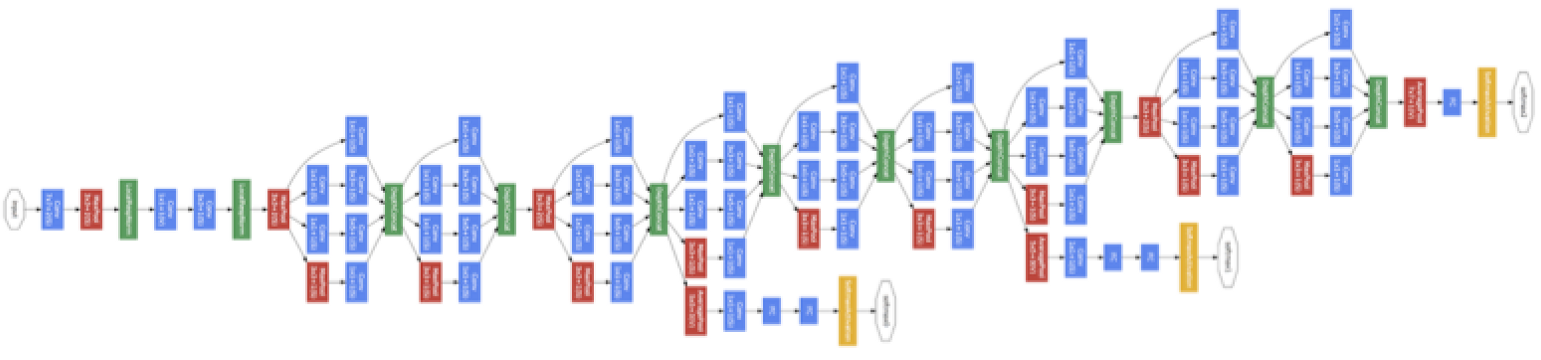
\includegraphics[width=0.8\textwidth]{./figures/inception-network.png}
\end{center}

\begin{columns}
\begin{column}{0.4\textwidth}
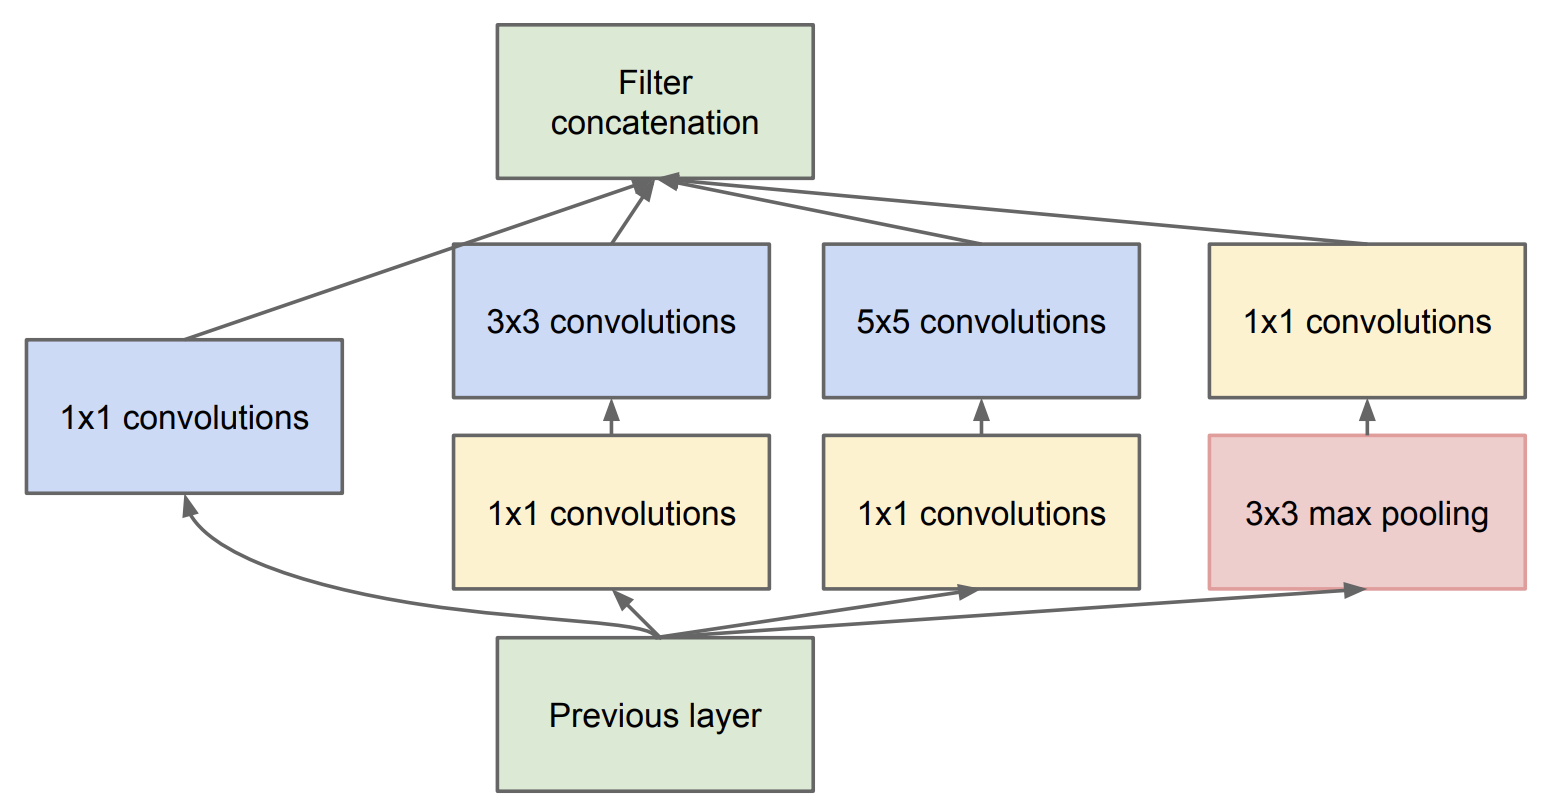
\includegraphics[width=1.11\textwidth]{./figures/inception-module.png}\\
define multi-branch blocks
\end{column}
\begin{column}{0.55\textwidth}
\begin{itemize} \is{2mm}
\item use $1\times 1$ convolutions to \textbblue{reduce dimensionality}
\item adapt dimensionality to size of downstream filter window
\item allows for increasing width (dim reduce) and depth (net-in-net)
% \item multiple processing paths
\end{itemize}
\end{column}
\end{columns}
\end{frame}



%%%%%%%%%%%%%%%%%%%%%%%%%%%%%%%%%%%%%%%%
\begin{frame} \frametitle{Residual Networks: ResNets}
%%%%%%%%%%%%%%%%%%%%%%%%%%%%%%%%%%%%%%%%
\begin{columns}
\begin{column}{0.58\textwidth}
{\small \textit{He, Zhang, Ren, Sun: Deep residual learning for image recognition. CVPR 2016. [23k+cit]}}
\end{column}
\begin{column}{0.40\textwidth}
\begin{center}
\includegraphics[width=0.79\textwidth]{./figures/shortcut}\\[3mm]
\includegraphics[width=1.12\textwidth]{./figures/shortreduce}
\end{center}
\end{column}
\end{columns}
\vspace*{3mm}

\begin{itemize} \is{2mm}
\item learn changes to the \textbblue{identity map} (aka.~shortcut connections) 
\item use small filters (VGG), use dimension reduction (inception)
\item reach depth of $100+$ layers (+increase accuracy +trainable)
\end{itemize}
\end{frame}

%%%%%%%%%%%%%%%%%%%%%%%%%%%%%%%%%%%%%%%%
\begin{frame} \frametitle{Other Themes \& Ideas}
%%%%%%%%%%%%%%%%%%%%%%%%%%%%%%%%%%%%%%%%
\setlength{\tabcolsep}{2pt}

\begin{columns}
\begin{column}{0.55\textwidth}
{\small \textit{Huang et al.: Densely connected convolutional networks. CVPR 2017.  [3.8k+cit]}}
\end{column}
\begin{column}{0.50\textwidth}
%\begin{itemize}
%\item 
connect all previous layers to next 
% \end{itemize}
\includegraphics[width=1.0\textwidth]{./figures/densenet}
\end{column}
\end{columns}

\vspace*{4mm}
\begin{columns}
\begin{column}{0.55\textwidth}
{\small Zagoruyko, Komodakis: Wide residual networks. BMCV 2016 \textit{[1.1k+cit]}}
\end{column}
\vspace*{2mm}

\begin{column}{0.50\textwidth}
% \begin{itemize}
% \item 
wide ResNets +dropout
%\end{itemize}
\includegraphics[width=0.9\textwidth]{./figures/wideres}
\end{column}
\end{columns}

\vspace*{4mm}
\begin{columns}
\begin{column}{0.55\textwidth}
{\small Jaderberg, Simonyan, Zisserman: Spatial transformer networks. NIPS 2015 \textit{[1.6k+cit]}}
\end{column}
\begin{column}{0.50\textwidth}
% \begin{itemize}
% \item 
parameterized transforms + spatial attention mechanism
% \end{itemize}
\includegraphics[width=0.7\textwidth]{./figures/spatialransform}
\end{column}
\end{columns}
\end{frame}

%%%%%%%%%%%%%%%%%%%%%%%%%%%%%%%%%%%%%%%%
\begin{frame} \frametitle{Squeeze-and-Excitation Networks}
%%%%%%%%%%%%%%%%%%%%%%%%%%%%%%%%%%%%%%%%
{\small \textit{Hu, Shen, Sun: Squeeze-and-excitation networks. \\CVPR 2018. [0.8k+cit]}}\\[1mm]

\begin{center}
\includegraphics[width=0.71\textwidth]{./figures/se}
\end{center}


\begin{itemize} \is{2mm}
\item learn dependencies between channels 
\item fixed per channel summarization (e.g.~spatial average)
\item gating mechanism that re-weights channels
\end{itemize}
\end{frame}



%%%%%%%%%%%%%%%%%%%%%%%%%%%%%%%%%%%%%%%%
%%%%%%%%%%%%%%%%%%%%%%%%%%%%%%%%%%%%%%%%
\section{Deep Generator Networks}
\frame{\sectionpage}
%%%%%%%%%%%%%%%%%%%%%%%%%%%%%%%%%%%%%%%%
%%%%%%%%%%%%%%%%%%%%%%%%%%%%%%%%%%%%%%%%


% ----------------------------------------------------------------------------
\begin{frame}
\frametitle{
%%%%%%%%%%%%%%%%%%%%%
Deep Generative Mechanisms
%%%%%%%%%%%%%%%%%%%%%
}
Key idea: use power of DNNs to create \textbblue{complex distributions}\\[4mm]
\begin{itemize}\is{4mm}
\item input random source: $\Re^m \ni \z \sim \mathcal N(0,\mathbf I)$ 
\item transform (deterministically) through DNN $F_\theta: \Re^m \to \Re^n$ 
\item induces $\theta$-parameterized distribution over $\Re^n$
\item expectations $\E_\x[g(\x)] = \E_\z\left[ g(F_\theta(\z)) \right]$ \\[1mm] = \textbblue{law of the unconscious statistician}
\end{itemize}
\end{frame}

% ----------------------------------------------------------------------------
\begin{frame}
\frametitle{
%%%%%%%%%%%%%%%%%%%%%
Deep Generative Mechanisms: Learning Signal
%%%%%%%%%%%%%%%%%%%%%
}
Key challenge: how to derive a learning signal?\\[2mm]
\begin{itemize}\is{2mm}
\item na\"ively: use maximum likelihood estimation? -- intractable!
\item learn inference network and use lower bound approximation (\textbblue{variational autoencoder})
\begin{align*}
\theta \stackrel{\text{max}}\longrightarrow \underbrace{\log p_\theta(\x)}_{\text{intractable}} \ge \underbrace{\E_{q_\phi}\left[\log p_\theta(\x|\z) + \log \frac{p(\z)}{q_\phi(\z|\x)} \right]}_{\text{tractable MC gradients}}
\stackrel{\text{max}}\longleftarrow \theta 
\end{align*}
\item use implicit discriminator loss (\textbred{generative adversarial net})
\begin{align*}
\theta \stackrel{\text{max}}\longrightarrow  \inf_\phi \ell(\phi,\theta)
\end{align*}
$\ell(\phi,\theta)$: discriminative loss b/w true and $\theta$-generated samples
\end{itemize}
\end{frame}

%%%%%%%%%%%%%%%%%%%%%%%%%%%%%%%%%%%%%%%%
\begin{frame} \frametitle{Deep Convolutional Generative Adversarial Networks}
%%%%%%%%%%%%%%%%%%%%%%%%%%%%%%%%%%%%%%%%
{\small \textit{Radford, Metz, Chintala: Unsupervised representation learning with deep convolutional generative adversarial networks. ICLR 2016 [3.6k+cit]}}
\begin{center}
\includegraphics[width=0.7\textwidth]{figures/dcgan}
\end{center}
\begin{columns}
\begin{column}{0.25\textwidth}
\includegraphics[width=1\textwidth]{figures/bedrooms}
\end{column}
\begin{column}{0.68\textwidth}
\begin{itemize}\is{1mm}
\item running ConvNet in reverse mode
\item many tricks to make work!
\item cf.~{\small \textit{Salimans et al: Improved Techniques for Training GANs, NIPS 2016 [1.8k+cit]}}
\item cf.~{\small \textit{Brock et al.: Large scale GAN training for high fidelity natural image synthesis 2018}}
\end{itemize}
\end{column}
\end{columns}
\end{frame}


%%%%%%%%%%%%%%%%%%%%%%%%%%%%%%%%%%%%%%%%
\begin{frame} \frametitle{Fast Cosmic Web Simulations with GANs}
%%%%%%%%%%%%%%%%%%%%%%%%%%%%%%%%%%%%%%%%
{\small \textit{Rodriguez, Kacprzak, Lucchi, Amara,  Sgier, Fluri, Hofmann, R\'efr\'egier: Fast cosmic web simulations with generative adversarial networks. Computational Astrophysics and Cosmology 2018 [0.009k cit ;-)]}}
\begin{columns}
\begin{column}{0.6\textwidth}
\begin{center}
\includegraphics[width=0.9\textwidth]{figures/cosmogan}
\end{center}
\end{column}
\begin{column}{0.35\textwidth}
cf.~talk by Nathana\"el Perraudin on Tuesday
\end{column}
\end{columns}
\end{frame}

%%%%%%%%%%%%%%%%%%%%%%%%%%%%%%%%%%%%%%%%
\begin{frame} \frametitle{Photorealistic Image Generation}
%%%%%%%%%%%%%%%%%%%%%%%%%%%%%%%%%%%%%%%%
{\small \textit{Karras, Laine, Aila: A style-based generator architecture for generative adversarial networks. CVPR 2019}}\\[1mm]

\begin{columns}
\begin{column}{0.40\textwidth}
\begin{center}
\includegraphics[width=0.95\textwidth]{figures/styleGAN}
\end{center}
\end{column}
\begin{column}{0.57\textwidth}
\begin{itemize}\is{2mm}
\item Globally map Gaussian noise +locally affine
\item Inject randomness at different resolutions
\item Adaptive instance normalization
\begin{align*}
\tilde x[s,t]=g[s,t] \frac{x[s,t] - \mu}{\sigma} + b[s,t]
\end{align*}
\end{itemize}
\end{column}
\end{columns}
\end{frame}

%%%%%%%%%%%%%%%%%%%%%%%%%%%%%%%%%%%%%%%%
\begin{frame} \frametitle{Photorealistic Image Generation: Human Faces}
%%%%%%%%%%%%%%%%%%%%%%%%%%%%%%%%%%%%%%%%
\begin{center}
\includegraphics[width=0.540\textwidth]{figures/faces}
\end{center}
\end{frame}


%%%%%%%%%%%%%%%%%%%%%%%%%%%%%%%%%%%%%%%%
\begin{frame} \frametitle{Image-to-Image Translation (pix2pix)}
%%%%%%%%%%%%%%%%%%%%%%%%%%%%%%%%%%%%%%%%
{\small \textit{Isola, Zhu, Zhou, Efros: Image-to-image translation with conditional adversarial networks. CVPR 2017. [2.3k+cit]}}\\[1mm]

\begin{center}
\includegraphics[width=0.75\textwidth]{figures/unet}
\end{center}

\begin{itemize}\is{2mm}
\item Use U-net style skip connections (+++)\\[3mm]
\item Condition GAN discriminator on input (+++)
\item PatchGAN: discriminator w/ $\approx 70 \times 70$ pixel patches (++)
\item Combine GAN objective with $L_1$ distance (++)
\end{itemize}
\end{frame}

%%%%%%%%%%%%%%%%%%%%%%%%%%%%%%%%%%%%%%%%
\begin{frame} \frametitle{Semantically-Conditioned Image Synthesis: SPADE}
%%%%%%%%%%%%%%%%%%%%%%%%%%%%%%%%%%%%%%%%
{\small \textit{Park, Liu, Wang, Zhu: Semantic Image Synthesis with Spatially-Adaptive Normalization. CVPR 2019 [?+cit]}}\\[1mm]

\begin{columns}
\begin{column}{0.4\textwidth}
\begin{center}
\includegraphics[width=0.85\textwidth]{figures/spade}\\[3mm]
\includegraphics[width=1\textwidth]{figures/spadeall}
\end{center}
\end{column}
\begin{column}{0.599\textwidth}
\begin{itemize}\is{2mm}
\item Normalized activations are denormalized by modulating with learned affine transformation (external data)
\item Example: condition on semantic segmentation mask
\item Multiresolution architecture 
\end{itemize}
\end{column}
\end{columns}
\end{frame}

%%%%%%%%%%%%%%%%%%%%%%%%%%%%%%%%%%%%%%%%
\begin{frame} \frametitle{SPADE: Results}
%%%%%%%%%%%%%%%%%%%%%%%%%%%%%%%%%%%%%%%%
\begin{center}
\includegraphics[width=1.06\textwidth]{figures/spade1}
\end{center}
\end{frame}

%%%%%%%%%%%%%%%%%%%%%%%%%%%%%%%%%%%%%%%%
%%%%%%%%%%%%%%%%%%%%%%%%%%%%%%%%%%%%%%%%
\section{Conclusion}
\frame{\sectionpage}
%%%%%%%%%%%%%%%%%%%%%%%%%%%%%%%%%%%%%%%%
%%%%%%%%%%%%%%%%%%%%%%%%%%%%%%%%%%%%%%%%

%%%%%%%%%%%%%%%%%%%%%%%%%%%%%%%%%%%%%%%%
\begin{frame} \frametitle{Conclusions \& Outlook}
%%%%%%%%%%%%%%%%%%%%%%%%%%%%%%%%%%%%%%%%
\begin{enumerate}\is{4mm}
\item Promising successes with ConvNets in Cosmology (also in backward mode!)
\item Utilize additional improvements developed by ML/DL community 
\item Find more use cases / make more integrated use of DNNs
\item Generative models: understand how they learn to shortcut expensive physics-based simulations!
\end{enumerate}
\end{frame}

\bibliography{th}
\bibliographystyle{acm}


\end{document}
